\part{Concepts théoriques}
\chapter{Monochronique et Polychronique}
\paragraph{}
D'après Edward Twitchell Hall, un antropologue américain et spécialiste de l'interculturalité, chaque culture a ses propres spécificités. En effet, dans toutes les cultures il ya un mode de fonctionnement différent lorsque nous évoquons les termes de délai de réalisation, de ponctualité, de rythme ou de perception d'un évènement.
\paragraph{}
Nous pouvons différencier deux cultures majeurs différentes: le temps monochronique et polychronique.
\paragraph{}
Concernant les caractéristiques du temps monochronique, on peut distinguer le fait que les personnes issus de cette culture font généralement une chose à la fois. Par exemple au travail, un employé désirant qu'on l'aide pour une tâche devra attendre que la personne à qui il demande finisse sa tâche avant de l'aider. On peut remarquer cette différence de culture dans les multinationales qui emploient plusieurs nationalités. Etre sensibilisé à cette différence de culture permet de mieux appréhender ses collègues et éventuellement être tolérant envers eux.
\paragraph{}
Au contraire, les personnes issus de la culture polychronique auront tendance à se dispersé en faisant plusieurs tâches simultanément. En effet, ils ressentent une charge affective qui les oblige à céder la priorité aux relations personnelles plutôt que les relations d'affaires. Ils aiment échanger de l'information pour apprendre à se connaitre.
\paragraph{}
La culture monochronique prône le dicton "`le temps c'est de l'argent"' et valorise donc la ponctualité et le respect des programmes établis. L'objectif est d'être performant. Les personnes issus de la culture monochronique sont contre toute interuption de leurs travails qui briseraient les actions. Concernant le domaine privé, leurs relations sont généralement superficielles.

\chapter{Communication haut contexte et bas contexte}

\chapter{Sphères publiques et privées}

\chapter{4 dimensions culturelles}
\paragraph{}
Geert Hofstede est un psychologue anthropologue hollandais qui a étudié les interactions entre les différentes cultures, il est le référent dans le management interculturel. Un jour IBM lui a demandé de prouver qu’il y avait une forte culture d’entreprise chez eux. Pour cela, il a créé une théorie basée sur 4 dimensions culturelles et en a tiré un questionnaire à choix multiple auquel tous les employés ont répondu pour déterminer la force de leur culture d’entreprise.
\paragraph{}
Les quatre dimensions culturelles sont la distance hiérarchique, l’individualisme, le contrôle d’incertitude et le niveau de masculinité/féminité.

\section{distance hiérarchique}
\paragraph{}
La distance hiérarchique consiste au pouvoir fourni à une personne face à ses subordonnés. En effet, dans un pays à forte distance hiérarchique, les subordonnés ne doivent pas dire ce qu’ils pensent, ils doivent juste faire ce qu’on leur dit. Par exemple, à la Cafeteria, lorsqu’il y a des étudiants en train de faire la queue pour acheter un café, les professeurs ont tendances à leur passer devant. Il s’agit ici d’une démonstration de forte hiérarchie : même si les étudiants trouvent cette attitude immorale, ils se taisent et prennent sur eux. Dans une culture à faible distance hiérarchique, il est normal de contredire son supérieur si l’on n’est pas d’accord. 

\section{individualisme}
\paragraph{}
L’individualisme consiste à valoriser la pensée personnelle. De ce fait, dans une culture à fort individualisme, il est normal et valorisant de dire ce qu’on pense et de réfléchir par soi-même. Au contraire, dans une culture à fort collectivisme, la pensée de la collectivité est valorisée : la collectivité est plus importante que l’individu. Il y a donc un lien entre distance hiérarchique et individualisme. En effet, si l’on n’est pas d’accord avec son supérieur on peut le contredire sans problème dans une culture individualiste. Une culture individualiste a donc une faible distance hiérarchique.
\paragraph{}
Cependant, la France possède une forte distance hiérarchique bien que ce soit une culture individualiste. En effet, les français peuvent contredire leur chef s’ils ne sont pas d’accord mais le chef aura le dernier mot. 

\section{Contrôle d'incertitude}
\paragraph{}
Une culture à haut contrôle d’incertitude mettra tout en place pour éviter les choses inattendues tandis qu’une culture à bas contrôle d’incertitude sait très bien s’adapter face à l’inattendue puisqu’elle ne met pas énormément de choses en place pour éviter celui-ci.  Ainsi, une culture à haut contrôle d’incertitude sera normative : beaucoup de normes seront inventées pour éviter de se trouver face à un inconnu. Une culture à bas contrôle d’incertitude sera plus pragmatique : l’inattendu fait partie de la vie, c’est ce qui la rend intéressante, il n’est donc pas nécessaire de l’éviter à tout prix. 

\section{Masculinité/Féminité}
\paragraph{}
Le niveau de masculinité d’une culture dépend des valeurs valorisées par cette culture. Une culture masculine valorise le succès et la réussite tandis qu’une culture féminine valorise la modestie et la compassion pour les plus pauvres et ceux qui ont moins bien réussi dans leur vie. Par exemple, le Japon et l’Allemagne sont des cultures à fort niveau de masculinité tandis que la France et la Suède sont des cultures à fort niveau de féminité. 

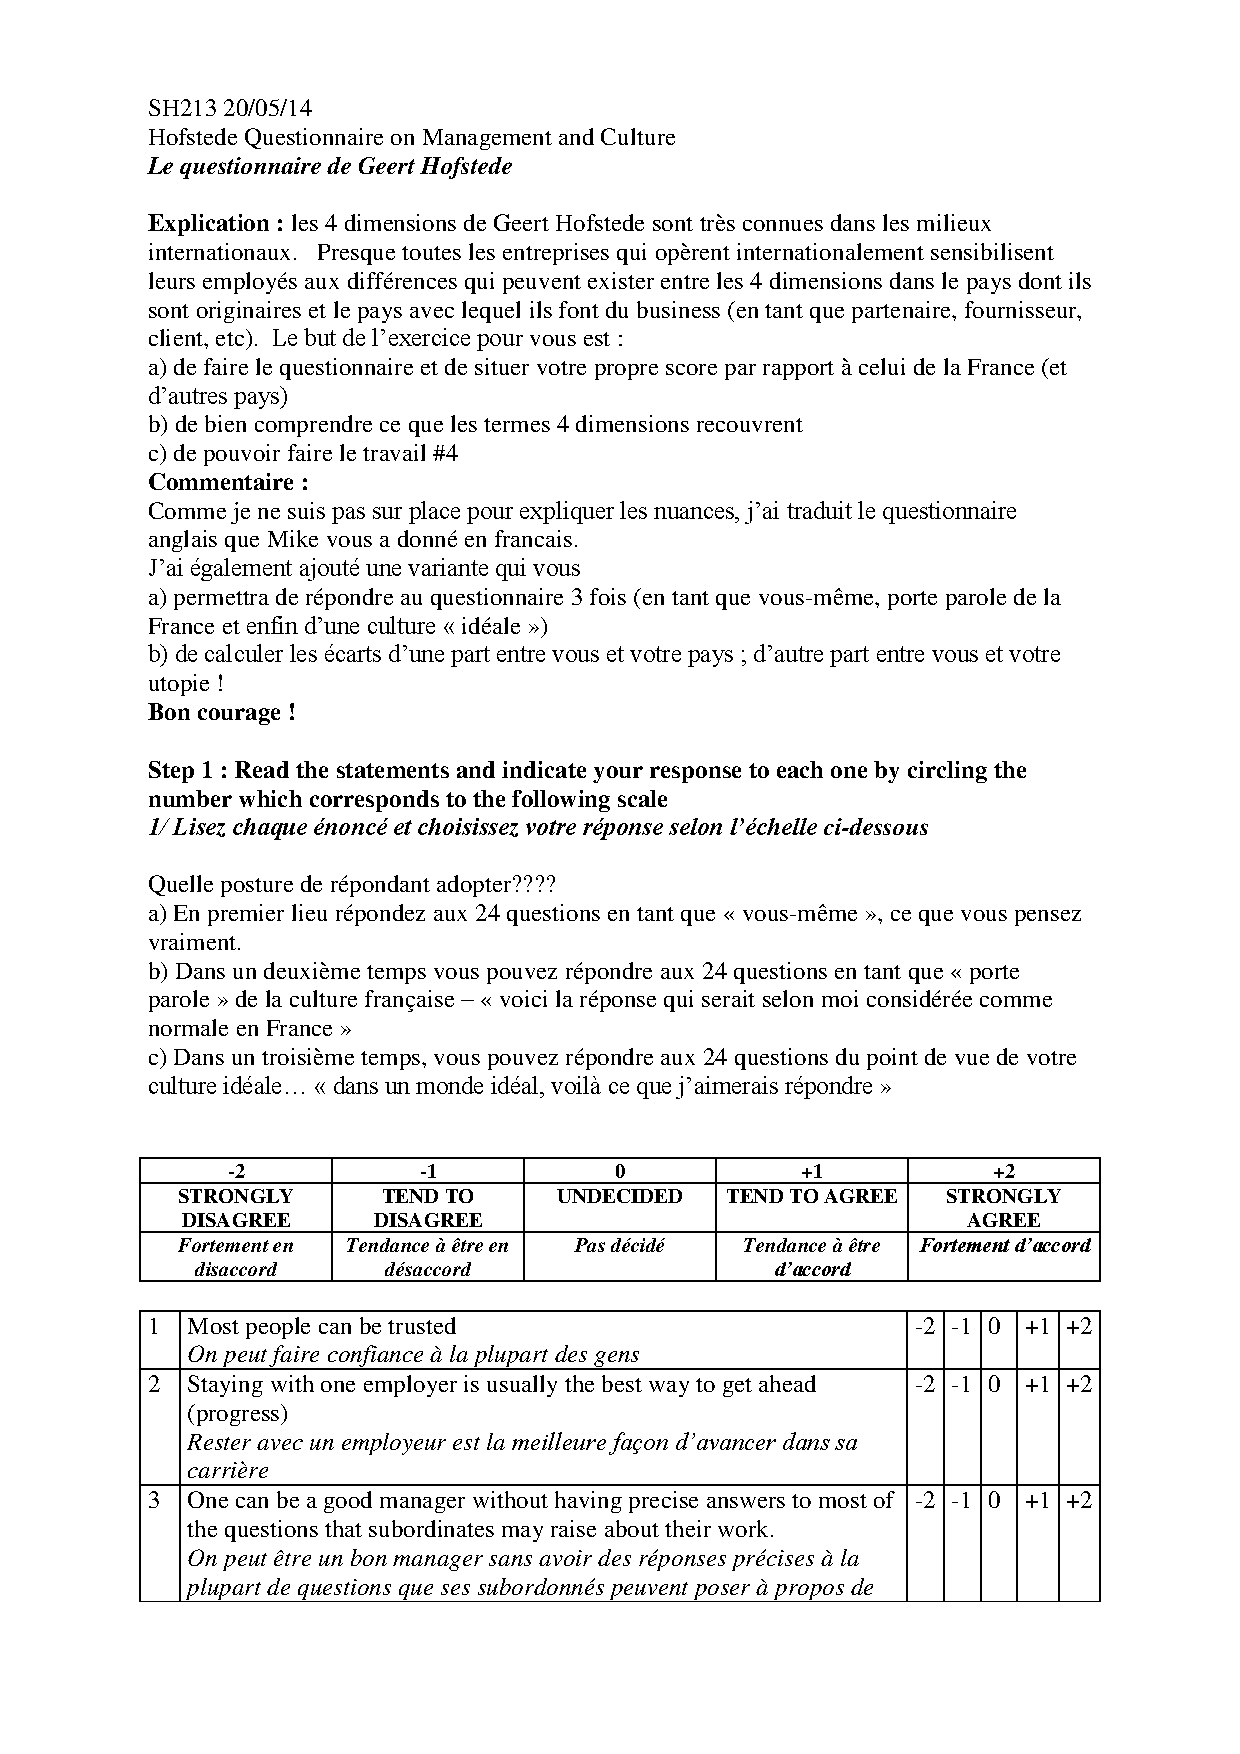
\includepdf[pages = {1-6}]{hofstedequestfrancais.pdf}